\documentclass[12pt]{article}
\usepackage{geometry}
\geometry{margin=5mm}
\usepackage{graphicx}

\makeatletter
\renewcommand \dotfill {\leavevmode \cleaders \hb@xt@ 5mm{\hss .\hss }\hfill \kern \z@}
\makeatother

\begin{document}
    \section*{6N5P}
    \subsection*{Double triode with individual cathodes}
    
    \par
    \begin{minipage}[b][0mm][t]{0.45\textwidth}
        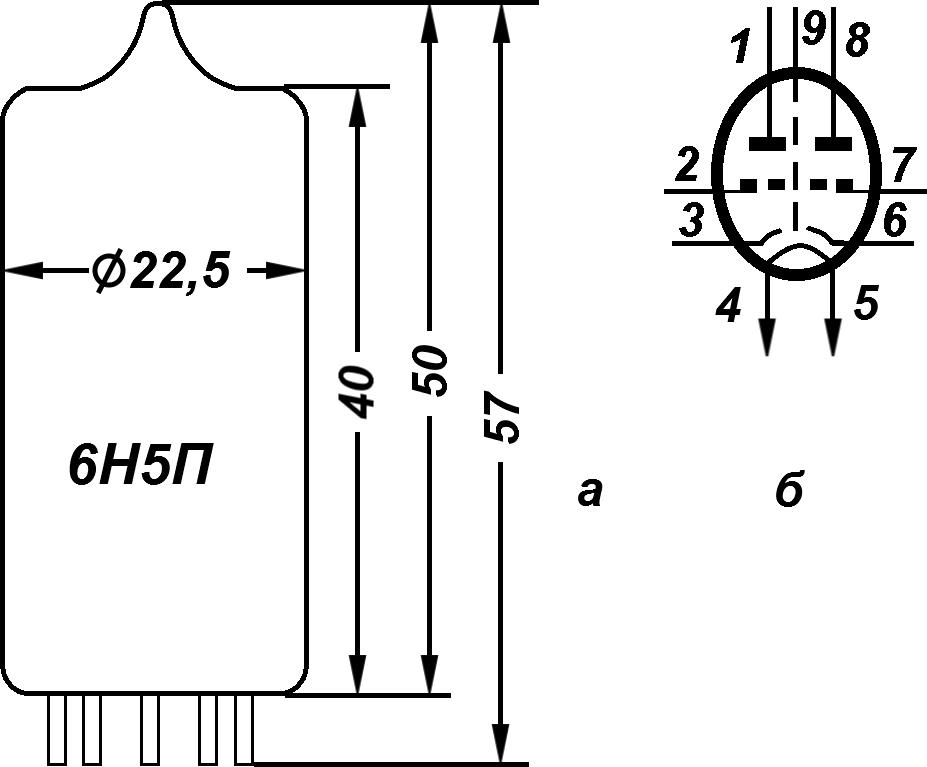
\includegraphics[width=80mm]{symbol.png}
    \end{minipage}
    \begin{minipage}[b][0mm][t]{0.45\textwidth}
        \begin{raggedright}
            \quad Intended for amplification of high frequency voltage in schemes of automatic gain control.
            \vspace{2mm}
            \hrule
            \vspace{2mm}
            Figure 326, Lamp 6N5P:
            \vspace{-4mm}
            \begin{itemize} \setlength \itemsep{-2.25mm}
                \item[a] --- Basic dimensions
                \item[b] --- Schematic symbol
                \item[1] --- Anode of the first triode
                \item[2] --- Grid of the first triode
                \item[3] --- Cathode of the first triode
                \item[4 \& 5] --- Heater
                \item[6] --- Anode of the second triode
                \item[7] --- Grid of the second triode
                \item[8] --- Cathode of the second triode
                \item[9] --- Screen
            \end{itemize}
        \end{raggedright}
    \end{minipage}
    
    \vspace{70mm}
    
    \begin{tabular}{l@{}}
        Indirectly heated cathode. \\
        Works in any position. \\
        Available in glass finger design. \\
        Service life not less than 500 hours. \\
        9-pin base with a button bottom. \\
    \end{tabular}
    
    \vspace{3mm}
    \hspace{-7mm} \textbf{Inter-electrode capacitance}
    \vspace{3mm}
    
    \begin{tabular}{p{105mm}l@{}l}
        Input of each triode \hspace{-2.7mm} \dotfill & & 3nF \\
        Output of the first triode \hspace{-2.3mm} \dotfill & & 1.5nF \\
        Output of the second triode \hspace{-2.1mm} \dotfill & & 1.7nF \\
        Passage of each triode \hspace{-1.7mm} \dotfill & & 2.25nF \\
        Between each anode \hspace{-3.1mm} \dotfill & \hspace{-1.0mm} less than \hspace{1mm} & 0.2nF \\
    \end{tabular}
    
    \vspace{3mm}
    \hspace{-7mm} \textbf{Electrical ratings}
    \vspace{3mm}
    
    \begin{tabular}{p{105mm}l@{}l}
        Filament voltage \hspace{-2.0mm} \dotfill & & 6.3V \\
        Anode voltage \hspace{-2.6mm} \dotfill & & 200V \\
        Cathode automatic bias resistance \hspace{-3.8mm} \dotfill & & 600$\Omega$ \\
        Filament current \hspace{-2.1mm} \dotfill & & 600mA $\pm$50mA \\
        Anode current \hspace{-2.6mm} \dotfill & \hspace{-7mm} greater than \hspace{1mm} & 8mA \\
        Steepness characteristics \hspace{-0.9mm} \dotfill & & 4.2mA/V \\
        Gain \hspace{-0.4mm} \dotfill & & 27 \\
    \end{tabular}
    
    \vspace{1mm}
    \hspace{-7mm} \rule{25mm}{0.5mm}
    
    * When lamp is locked (anode current is 5 $\mu$A)
    
    \newpage
    
    \noindent \textbf{Absolute maximum ratings} \\
    (for each triode)
    
    \vspace{3mm}
    
    \begin{tabular}{p{105mm}l@{}l}
        Max filament voltage \hspace{0.0mm} \dotfill & \hspace{19mm} & 7V \\
        Min filament voltage \hspace{0.8mm} \dotfill & & 5.7V \\
        Max anode voltage \hspace{-1.1mm} \dotfill & & 300V \\
        Max anode power \hspace{1.2mm} \dotfill & & 2.2(vm,mW?) \\
        Max cathode current \hspace{0.4mm} \dotfill & & 25mA \\
        Max voltage between cathode and heater \hspace{-1.1mm} \dotfill & & 250V \\
        Max leakage current between cathode and heater \hspace{-5.5mm} \dotfill & & 20$\mu$A \\
        Min cathode automatic bias resistance \hspace{-1.3mm} \dotfill & & 600$\Omega$ \\
        Max grid resistance \hspace{-2.1mm} \dotfill & & 1M$\Omega$ \\
    \end{tabular}
    
    \vspace{5mm}
    \hspace{-5mm}
    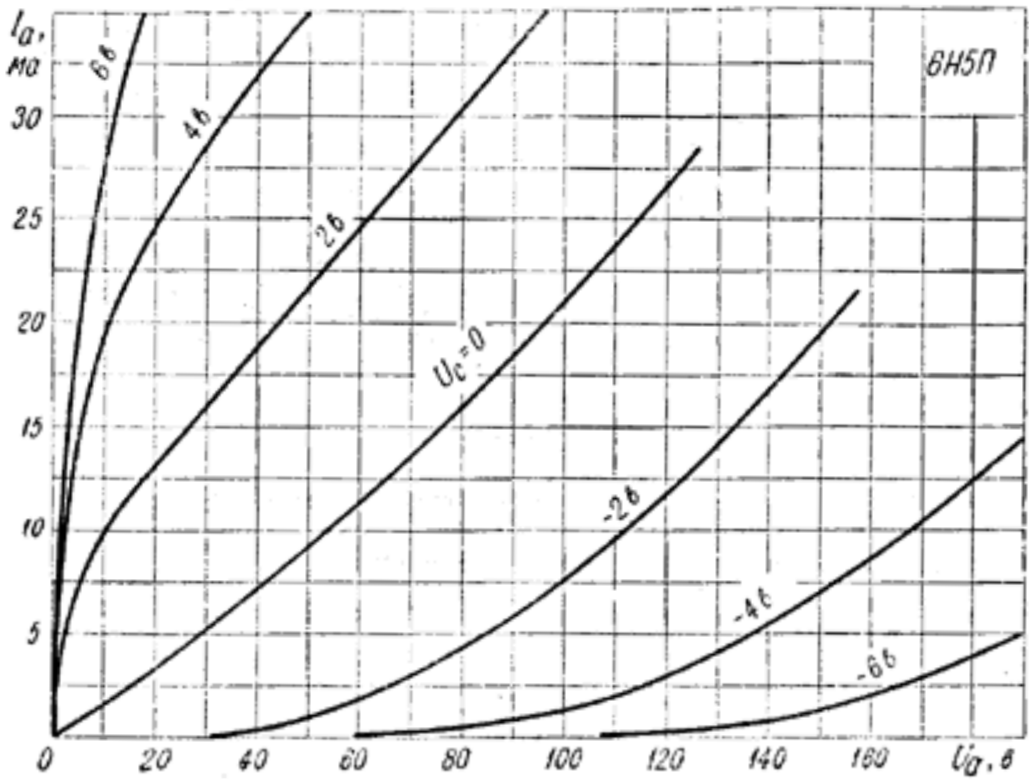
\includegraphics[width=200mm]{graph.png}
    
    Figure 327, averaged characteristics of anode current versus anode voltage.
\end{document}